\subsection{Example Game}
\label{sub:example_game}

MicroNet provides a simple but complete example of an \og{}. Although the sample
game is very simple it gives a good overview over the functionality of MicroNet.

The sample game is a guessing game which is played in rounds of 15 seconds.
In each round the players have to guess a number between 1 and 100. The players
receive a score based on the proximity of the guess to the number. The score of
all player is shown in a scoreboard. 

The game client of the sample game is a standalone Java application using the
Laterna console gui library. Laterna allows to develop window based GUIs for the
terminal. This allows to run the game client also on server environments
through the command line. \todo{screenshot}

\autoref{fig:sample_game_flow} shows the communication of the sample game. The
numeric sequence is the communication flow of a player vote and the capital
letter sequence is the round control communication.\\

\begin{figure}
	\centering
	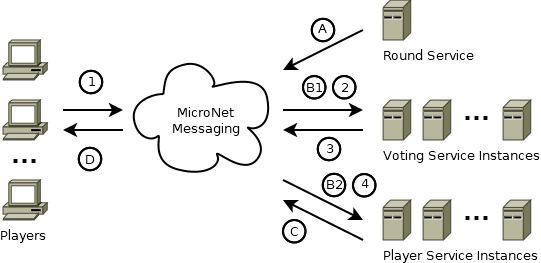
\includegraphics[width=\textwidth]{images/architecture/SampleGame}
	\caption{Communication flow of the Example Game.}
	\label{fig:sample_game_flow}
\end{figure}

The round control communication flow:

\begin{enumerate}[label=\Alph*.]
  \item The round service broadcasts a new new round event. The new round event
  contains the guessed number for the next round.
  \item \begin{enumerate}[label=\arabic*.]
    \item All voting services receive the new round event and store next the
    guess number in memory.
  	\item One player service receives the new round event to issue a score
  	broadcast. The scores of all players are available through the session store.
  \end{enumerate}
  \item The player service which received the new round event broadcasts a score
  update event to all participating players.
  \item Each player received the score update and updates its scoreboard
  accordingly.
   
\end{enumerate}

The player voting communication flow:

\begin{enumerate}
  \item The player sends his vote to the game application.
  \item The voting service instances compete for the vote messages.
  \item The processing voting service instance sends a score update message to
  an arbitrary player service.
  \item The processing player service persists the vote using the session store.
\end{enumerate}

It has to be mentioned that the round service is a singleton service. This is
necessary to ensure that the new round event is broadcast only once. Problems
like this are very common in distributed game development. To ensure the
stability of the application despite having singleton services can be quite a
challenge. One strategy is to keep singleton services as small as possible to
leave little room for failure. In the case of a failure the composition engine
must ensure that the singleton service is restarted. 

A singleton service must be designed in a way that no crucial data is lost upon
service failure and it must be possible to recover the state of a singleton
service after service failure.



